\chapter{Исследовательская часть}

В данном разделе исследуется влияние разных типов индексирования на время выполнения базовых операций с таблицей:
вставки, выборки и удаления. Цель --- показать, как выбор индекса влияет на производительность и скорость выполнения
основных операций

\section{Технические характеристики ЭВМ}

Все замеры проводились на ЭВМ, характеристики которой приведены
ниже:

\begin{itemize}
    \item процессор: AMD Ryzen™ 7--5800H with Radeon™ Graphics × 16, 3.8 ГГц~\cite{radeon};
    \item ОС: 64-разрядная операционная система Ubuntu 24.04.1 LTS~\cite{ubuntu};
    \item оперативная память: 16,0 ГБ;
    \item число логических ядер -- 16;
    \item СУБД: PostgreSQL.
\end{itemize}

\section{Постановка задачи}

Цель исследования — измерить зависимость времени выполнения \texttt{INSERT}, \texttt{SELECT} и \texttt{DELETE} от
используемого типа индексирования над столбцом \(k\) в одной и той же таблице.
Рассматриваемые сценарии:

\begin{enumerate}[label=\arabic*.]
  \item \textbf{Без индекса (Heap)} — таблица-куча без индексов
        (см. реализацию~\ref{lst:no-index}).
  \item \textbf{B-Tree} — некластерный индекс по атрибуту \(k\)
        (см. реализацию~\ref{lst:btree}).
  \item \textbf{UNIQUE B-Tree} — уникальный индекс по атрибуту \(k\)
        (см. реализацию~\ref{lst:uniq}).
  \item \textbf{CLUSTER по \(k\)} — кластеризованная (физически упорядоченная) укладка таблицы на основе B-Tree
        (см. реализацию~\ref{lst:cluster}).
\end{enumerate}

\begin{lstlisting}[language=SQL,caption={Сценарий без индекса},label={lst:no-index}]
type noIndex struct{ pool *pgxpool.Pool }

func (s noIndex) Name() string { return "heap_no_index" }
func (s noIndex) Prepare(ctx context.Context) {
    mustExec(ctx, s.pool, `DROP INDEX IF EXISTS idx_bench_k;`)
}
func (s noIndex) Reset(ctx context.Context) {
    mustExec(ctx, s.pool, `DROP INDEX IF EXISTS idx_bench_k;`)
}
func (s noIndex) PostInsertLayout(ctx context.Context) {
}
func (s noIndex) Cleanup(ctx context.Context) {
    mustExec(ctx, s.pool, `DROP INDEX IF EXISTS idx_bench_k;`)
}
\end{lstlisting}

\begin{lstlisting}[language=SQL,caption={Сценарий B-Tree по атрибуту k},label={lst:btree}]
type heapBtree struct{ pool *pgxpool.Pool }

func (s heapBtree) Name() string { return "heap_btree" }
func (s heapBtree) Prepare(ctx context.Context) {
    mustExec(ctx, s.pool, `DROP INDEX IF EXISTS idx_bench_k;`)
}
func (s heapBtree) Reset(ctx context.Context) {
    mustExec(ctx, s.pool, `DROP INDEX IF EXISTS idx_bench_k;`)
    mustExec(ctx, s.pool, `CREATE INDEX idx_bench_k ON bench_items(k);`)
}
func (s heapBtree) PostInsertLayout(ctx context.Context) {
    mustExec(ctx, s.pool, `ANALYZE bench_items;`)
}
func (s heapBtree) Cleanup(ctx context.Context) {
    mustExec(ctx, s.pool, `DROP INDEX IF EXISTS idx_bench_k;`)
}
\end{lstlisting}

\begin{lstlisting}[language=SQL,caption={Сценарий UNIQUE B-Tree по атрибуту k},label={lst:uniq}]
type heapUniqueBtree struct{ pool *pgxpool.Pool }

func (s heapUniqueBtree) Name() string { return "heap_unique_btree" }
func (s heapUniqueBtree) Prepare(ctx context.Context) {
    mustExec(ctx, s.pool, `DROP INDEX IF EXISTS idx_bench_k;`)
}
func (s heapUniqueBtree) Reset(ctx context.Context) {
    mustExec(ctx, s.pool, `DROP INDEX IF EXISTS idx_bench_k;`)
    mustExec(ctx, s.pool, `CREATE UNIQUE INDEX idx_bench_k ON bench_items(k);`)
}
func (s heapUniqueBtree) PostInsertLayout(ctx context.Context) {
    mustExec(ctx, s.pool, `ANALYZE bench_items;`)
}
func (s heapUniqueBtree) Cleanup(ctx context.Context) {
    mustExec(ctx, s.pool, `DROP INDEX IF EXISTS idx_bench_k;`)
}
\end{lstlisting}

\begin{lstlisting}[language=SQL,caption={Сценарий с укладкой CLUSTER по k},label={lst:cluster}]
type clusteredBtree struct{ pool *pgxpool.Pool }

func (s clusteredBtree) Name() string { return "clustered_btree" }
func (s clusteredBtree) Prepare(ctx context.Context) {
    mustExec(ctx, s.pool, `DROP INDEX IF EXISTS idx_bench_k;`)
}
func (s clusteredBtree) Reset(ctx context.Context) {
    mustExec(ctx, s.pool, `DROP INDEX IF EXISTS idx_bench_k;`)
    mustExec(ctx, s.pool, `CREATE INDEX idx_bench_k ON bench_items(k);`)
}
func (s clusteredBtree) PostInsertLayout(ctx context.Context) {
    mustExec(ctx, s.pool, `CLUSTER bench_items USING idx_bench_k;`)
    mustExec(ctx, s.pool, `ANALYZE bench_items;`)
}
func (s clusteredBtree) Cleanup(ctx context.Context) {
    mustExec(ctx, s.pool, `DROP INDEX IF EXISTS idx_bench_k;`)
}
\end{lstlisting}

\clearpage
\section{Результаты замеров}

В таблицах~\ref{tab:delete_median}--\ref{tab:select_median} представлены результаты измерения медианного времени (мс) от объёма \(N\)
для трёх операций и четырёх сценариев. Для каждого сценария и объема операций было выполнено 100 замеров.

\begin{table}[H]
\caption{Время выполнения операции удаления, в мс}
\label{tab:delete_median}
\begin{tabular}{|l|r|r|r|r|}
    \hline
Сценарий & кластер & некластер & без индекса & уник некластер\\
n &  &  &  &  \\
\hline
10000 & 102.77 & 105.50 & 59.07 & 103.61 \\
\hline
40000 & 312.88 & 312.83 & 189.67 & 314.87 \\
\hline
70000 & 532.92 & 528.74 & 318.15 & 535.05 \\
\hline
100000 & 749.52 & 763.72 & 447.66 & 759.35 \\
\hline
130000 & 953.86 & 1002.66 & 586.30 & 978.92 \\
\hline
160000 & 1170.91 & 1233.65 & 716.02 & 1207.56 \\
\hline
190000 & 1413.88 & 1465.53 & 843.07 & 1420.78 \\
\hline
\end{tabular}
\end{table}


\begin{table}[H]
\caption{Время выполнения операции вставки, в мс}
\label{tab:insert_median}
\begin{tabular}{|l|r|r|r|r|}
    \hline
Сценарий & кластер & некластер & без индекса & уник некластер\\
n &  &  &  &  \\
    \hline
10000 & 99.06 & 76.99 & 57.14 & 99.46 \\
    \hline
40000 & 306.83 & 306.55 & 184.22 & 307.66 \\
    \hline
70000 & 518.94 & 523.89 & 310.42 & 526.15 \\
    \hline
100000 & 734.69 & 754.65 & 435.56 & 742.64 \\
    \hline
130000 & 973.08 & 981.66 & 572.50 & 958.72 \\
    \hline
160000 & 1155.45 & 1221.09 & 699.15 & 1184.32 \\
    \hline
190000 & 1395.56 & 1443.21 & 822.09 & 1404.70 \\
    \hline
\end{tabular}
\end{table}


\begin{table}[H]
\caption{Время выполнения операции чтения, в мс}
\label{tab:select_median}
\begin{tabular}{|l|r|r|r|r|}
    \hline
Сценарий & кластер & некластер & без индекса & уник некластер\\
n &  &  &  &  \\
    \hline
10000 & 0.19 & 0.18 & 0.59 & 0.20 \\
    \hline
40000 & 0.26 & 0.34 & 1.89 & 0.36 \\
    \hline
70000 & 0.28 & 0.52 & 3.32 & 0.45 \\
    \hline
100000 & 0.28 & 0.53 & 4.67 & 0.51 \\
    \hline
130000 & 0.30 & 0.56 & 5.71 & 0.57 \\
    \hline
160000 & 0.27 & 0.58 & 7.05 & 0.56 \\
    \hline
190000 & 0.28 & 0.62 & 7.81 & 0.59 \\
    \hline
\end{tabular}
\end{table}


На рисунках~\ref{fig:insert}--\ref{fig:delete} представлена визуализация результатов:

\begin{figure}[H]
  \centering
  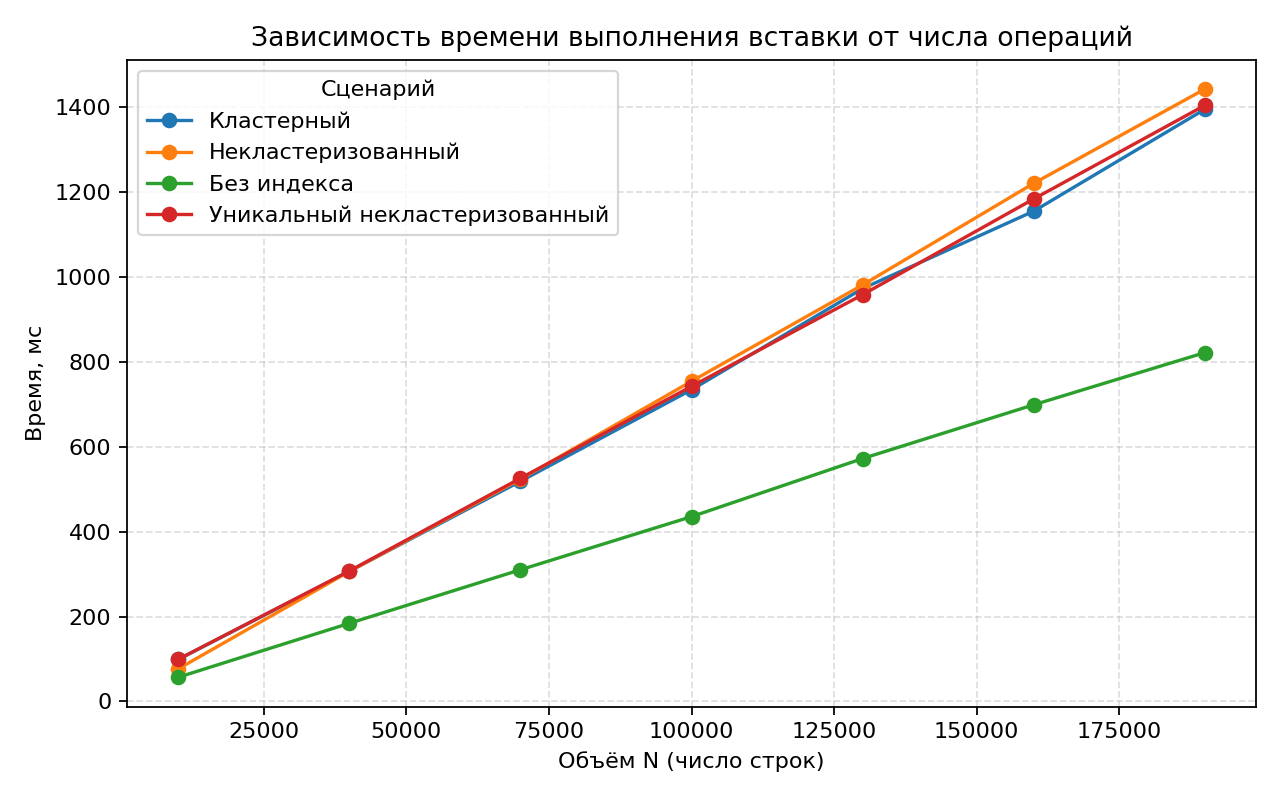
\includegraphics[width=\linewidth]{images/insert_line.png}
  \caption{Зависимость времени от числа операций вставки.}
  \label{fig:insert}
\end{figure}

\begin{figure}[H]
  \centering
  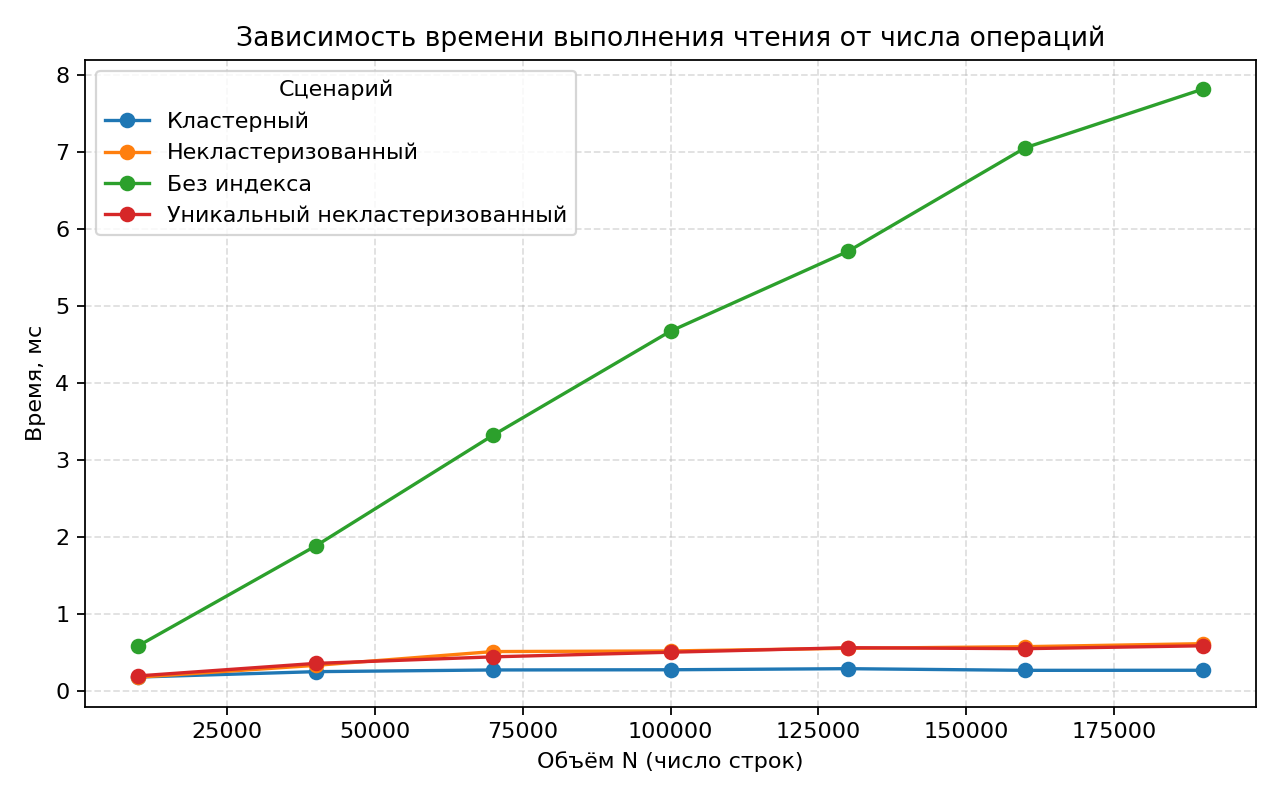
\includegraphics[width=\linewidth]{images/select_line.png}
  \caption{Зависимость времени от числа операций выбора.}
  \label{fig:select}
\end{figure}

\begin{figure}[H]
  \centering
  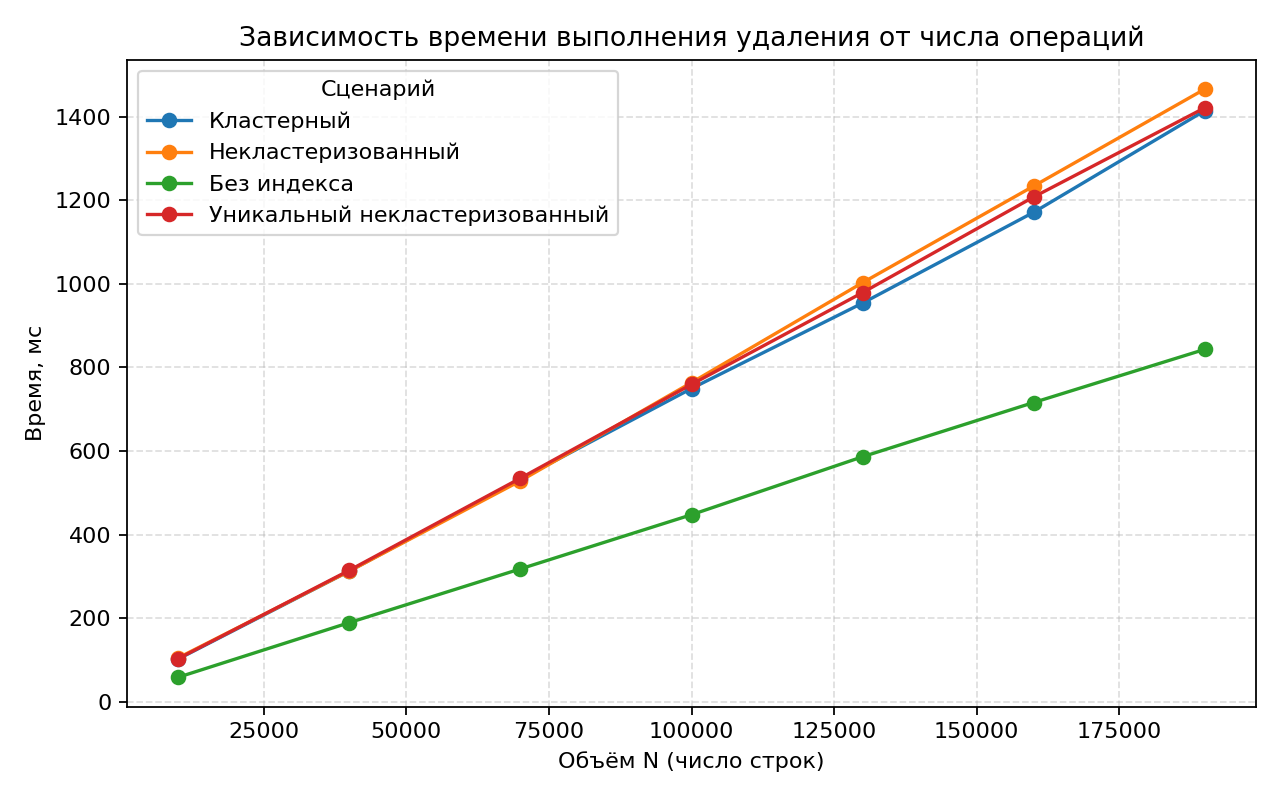
\includegraphics[width=\linewidth]{images/delete_line.png}
  \caption{Зависимость времени от числа операций удвления.}
  \label{fig:delete}
\end{figure}



\section*{Вывод}

В данном разделе описаны технические характеристики ЭВМ, на которой проводилось исследование,
а также представлены ход выполнения исследования и его результаты. Полученные данные подтвердили ожидания:
Время выполнения различных операций для разных типов индексов отличается.

Операция вставки выполняется быстрее примерно на 70\% при больших объемах данных, по сравнению с остальными сценариями.
Это объясняется тем, что без индекса записи просто добавляются в кучу,
тогда как для некластерных и уникальных индексов требуется дополнительное обновление бинарного дерева.
Уникальный индекс работает медленнее обычного, так как дополнительно проверяет уникальность ключей.

Аналогично, быстрее всего удаление происходит без индекса, примерно на 65\% по сравнению с остальными вариантами.
При наличии индекса, кроме пометки строк в куче, требуется удаление соответствующих ссылок из дерева,
что и увеличивает время. Разница между кластерным и некластерным индексами несущественна.

Наиболее заметный эффект индексы дают операции чтения: время выполнения с индексами остаётся
почти постоянным даже при росте $N$,
тогда как без индекса линейно увеличивается.
Кластеризация немного улучшает результаты по сравнению с индексами без кластеризации,
благодаря упорядоченному физическому размещению строк.
Уникальный индекс по скорости чтения сопоставим с обычным.

